\documentclass[a4paper,11pt]{article}
\usepackage[polish]{babel}
\usepackage[utf8]{inputenc}   % lub utf8
\usepackage[T1]{fontenc}
\usepackage{graphicx}
\usepackage{anysize}
\usepackage{enumerate}
\usepackage{times}
\usepackage{tikz}

%\marginsize{left}{right}{top}{bottom}
\marginsize{3cm}{3cm}{3cm}{3cm}
\sloppy
\begin{document}
\begin{figure}[!htb]
\centering
\begin{tikzpicture}
\node at (0,0) {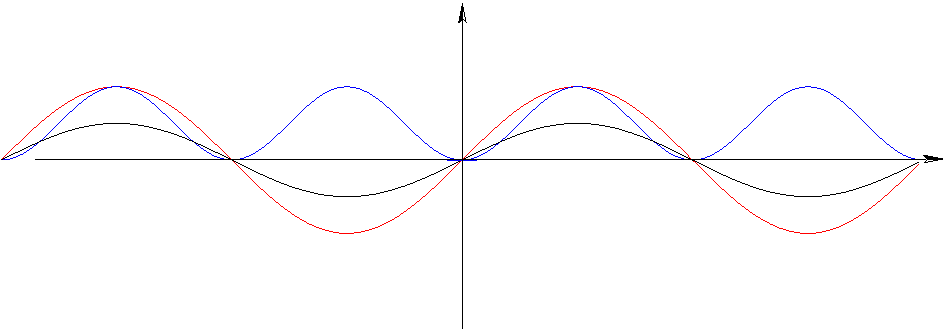
\includegraphics[scale=1]{f1.pdf}};
\node at (5.6,-1.5) {$f(x) = \sin(x)$};
\node at (5.6,1.5) {$g(x) = \sin^2(x)$};
\node at (2.0,0.5) {$h(x) = \frac{\sin(x)}{2}$};
\end{tikzpicture}
\caption{Wykresy funkcji}
\label{fig:funkcje}
\end{figure}
\end{document}